\documentclass[numbers=noenddot, a4paper, 12pt, headsepline, footsepline]{scrreprt}

% Deutsche Umlaute
\usepackage[utf8]{inputenc}

% deutsche Silbentrennung
\usepackage[ngerman]{babel}

%anführungszeichen
\usepackage[autostyle=true,german=quotes]{csquotes}

% Einbinden von Bildern
\usepackage{graphicx}

% Mathematische Pakete
\usepackage{amsmath}
\usepackage{amssymb}
\usepackage{amsfonts}
\usepackage{amsthm}
\usepackage{latexsym}
\usepackage{morefloats}
\usepackage{geometry} 


\usepackage{standalone}

% better looking tables
\usepackage{ifthen}
\usepackage{booktabs}
\usepackage{multirow}


% ausgabe von quelltext
\usepackage{textcomp}
\usepackage{listings}

%einbinden von pdf seiten
\usepackage{pdfpages}

\lstset{
	%	backgroundcolor=\color{lbcolor},
	tabsize=4,    
	%	rulecolor=,
	language=[GNU]C++,
	basicstyle=\scriptsize,
	upquote=true,
	%aboveskip={1.5\baselineskip},
	columns=fixed,
	showstringspaces=false,
	extendedchars=false,
	breaklines=true,
	%prebreak = \raisebox{0ex}[0ex][0ex]{\ensuremath{\hookleftarrow}},
	%frame=single,
	numbers=none,
	showtabs=false,
	showspaces=false,
	showstringspaces=false,
	identifierstyle=\ttfamily,
	language=C++,
	basicstyle=\ttfamily,
	keywordstyle=\color{blue}\ttfamily,
	stringstyle=\color{red}\ttfamily,
	commentstyle=\color[rgb]{0,.7,0}\ttfamily,
	morecomment=[l][\color{magenta}]{\#},
	%\lstdefinestyle{C++}{language=C++,style=numbers}’,
}
\lstset{
	basicstyle=\renewcommand{\baselinestretch}{.9}\ttfamily,
	xleftmargin=.5cm,
	language=C++,
	numbers=left,
	stringstyle=\color{black}\ttfamily,
	keywordstyle=\color{black}\ttfamily,
	numberstyle=\tiny}


% coolere referenzen
\usepackage[german]{fancyref}

%literatur mittels biber
\usepackage[backend=biber,
			style=alphabetic
			%citestyle=alphabetic 
			]{biblatex}

%\ExecuteBibliographyOptions{
%	sorting=nyt, %Sortierung Autor, Titel, Jahr
%	bibwarn=true, %Probleme mit den Daten, die Backend betreffen anzeigen
%}
\addbibresource{literatur.bib}

%querformat seiten
\usepackage{lscape}

%überschrift des Kapitel auf jeder Seite
\pagestyle{headings}

%lange tabellen mit seitenumbruch
\usepackage{longtable}

%abkürzungsverzeichnis
\usepackage{acronym}

%um links im pdf zu haben mit denen man hin und her springen kann
\usepackage{hyperref}

%%text farbig hinterlegen
%\usepackage{color}

%%um text durch, unter, über... streichen zu können
%\usepackage{ulem}

%um in tabellen zellen diagonal teilen zu können
%\usepackage{diagbox}


\begin{document}

%einbinden titelblatt
\title{Smart Car} 
\subtitle{Hauptseminar Projektstudium}
\author{\\
	\begin{tabular}{|c|c|c|}
		\hline 
		Knorr Thomas 		 & xyzk 	& HSP1 \\ 
		\hline 
		Lackner Andreas 	 & xyzk 	& HSP2 \\ 
		\hline 
		Schleinkofer Michael & xyzk 	& HSP2 \\ 
		\hline 
		Welker Franz 		 & 3119754  & HSP2 \\ 
		\hline 
		Wiche Fabian 		 & xyzk		& HSP1 \\ 
		\hline 
	\end{tabular} 
	}	

\date{\today}
%\clearpairofpagestyles

\makeatletter
\begin{titlepage}
	
	\begin{center}
		
\includegraphics[width=10cm]{./Images/OTHLogo.eps}\\
		\vspace{4cm}
		{\huge\bfseries\@title\unskip\strut\par}\paragraph{}
		{\Large\bfseries\@subtitle\unskip\strut\par}\paragraph{}
		An der\\
		Ostbayerischen Technischen Hochschule Regensburg\\
		Fakultät Informatik/Mathematik
		\paragraph{}
		Betreut durch Prof. Dr. Klaus Volbert\\
		\vspace{\fill}
		Vorgelegt von: \vspace{0,3cm}
		\@author\\
		\vspace{0,3cm}
		Datum: \@date
	\end{center}
\end{titlepage}
\makeatother



%arabische zahlen für seiten
\pagenumbering{arabic}

% Inhaltsverzeichnis anzeigen
%\parskip am schluss anpassen, so dass ein zweiseitiges inhaltsverzeichnis gut umgebrochen wird
{\parskip=+5mm \tableofcontents}

\chapter*{Einleitung}
 
Kurze Einleitung, warum haben wir uns das Thema ausgesucht (nicht lang oder so)...
Gibt z.B. Pace aber braucht man immer Handy, wollten es anders machen...











\chapter{Use Cases}
\label{sec:useCases}
Die Daten aus der OBD II Schnittstelle eines Autos, vereint mit dem GPS-Sensor und den anderen Sensoren des Dongles, bieten für eine Auswertung nahe zu unbegrenzte Möglichkeiten. Aus den Analysen entstehen Anwendungsfälle, für die sich das SmartCar System verwenden lässt. Das nachfolgende Kapitel beinhaltet eine Auswahl an Use Cases auf dessen Grundlage das Design und die Implementierung der einzelnen Komponenten entstanden ist.
\section{Aufzeichnen von Routen}
Ein Anwendungsbeispiel für SmartCar ist das Aufzeichnen von Routen während der der Fahrt. Der Dongle soll, nach dem Einstecken in die OBD-Schnittstelle, mithilfe des zusätzlichen GPS Moduls Fahrten aufzeichnen und auf einer SD-Karte speichern. Für jede Fahrt soll hier eine separate Datei erstellt werden. Zusätzlich zu den GPS-Koordinaten legt der Dongle noch ausgewählte Daten aus der OBD Schnittstelle auf der SD-Karte ab. Diese Aufzeichnung erfolgt so, dass eine Darstellung und Abspeicherung in einem externen System(Backend) möglich ist und dort auch einzelne Fahrten unterscheidbar sind.
\section{Analyse der aufgezeichneten Daten}
\label{Sec_AnayseDerAufgezeichnetenDaten}
Aus dem Abspeichern der oben genannten Informationen ergibt sich auch der zweite Anwendungsfall. Die Daten, die der Dongle abspeichert soll ein Backend anschaulich darstellen und Auswertungen über das Erfasste anfertigen. Solche Darstellungen sind z.B. Heat-maps, auf denen Daten wie Geschwindigkeit, Motordrehzahl oder Spritverbrauch für jede Fahrt zu sehen sind. So ist es möglich zu erkennen auf welchen Strecken wann welche Daten erfasst wurden. Ein Nutzer kann z.B. dann einsehen, wann er auf welchen Strecken wie viel Treibstoff verbraucht hat und dadurch seine Fahrgewohnheiten optimieren.
\section{Live Daten Anzeige von OBD Daten auf dem Smartphone}
Die vom Dongle erfassten Daten sind aber nicht nur für eine spätere Analyse interessant, sondern liefern auch während der Fahrt wertvolle Informationen. Aus diesem Grund ist ein weiterer Einsatzzweck das Darstellen von bestimmten Live-Daten auf einer Smartphone App. Die Kommunikation zwischen App und Smartphone erfolgt hier über Bluetooth Low Energy(BLE). Solche Live-Daten sind z.B. der aktuelle Verbrauch des Autos oder die derzeitige Geschwindigkeit. Das ist vor allem für ältere Autos interessant, da sie Daten wie Spritverbrauch meistens selbst noch nicht anzeigen. Aber auch Fahrer von neueren Autos können so die Ausgaben ihrer Autos mit denen der App vergleichen und etwaige Fehler im Fahrzeug erkennen
 
\chapter{System Design}
\begin{sidewaysfigure}
  \begin{center}
    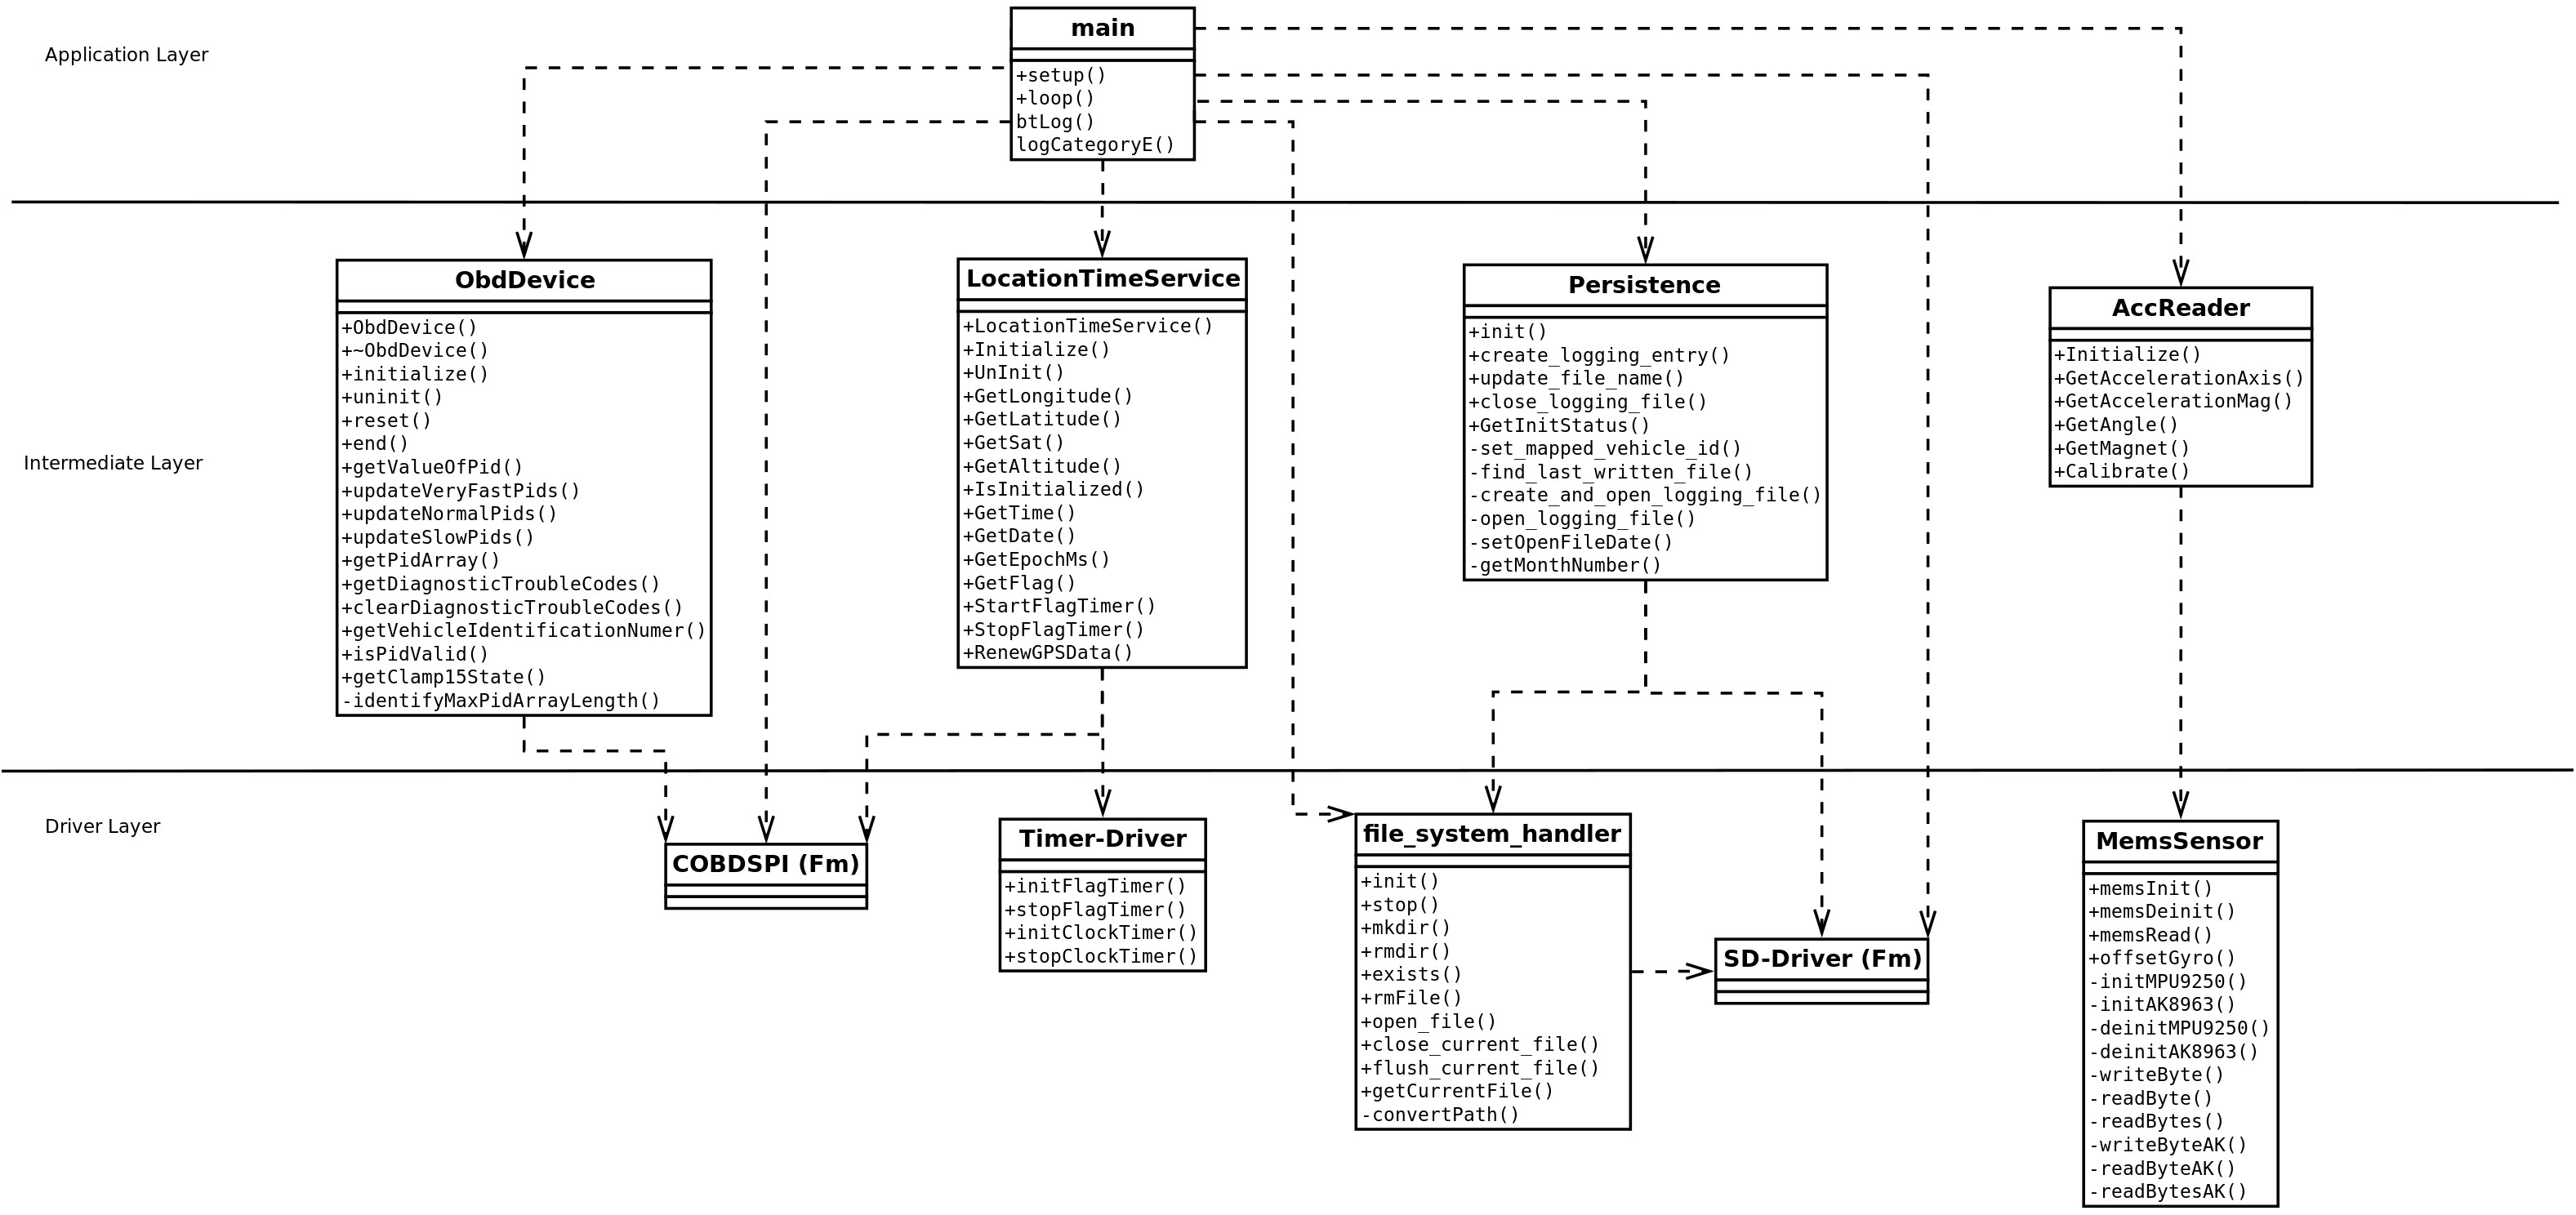
\includegraphics[width=\textwidth,height=15cm,keepaspectratio]{./img/Dongle_Arch_final}
    \caption{Architektur der Dongle-Software}
    \label{fig:dongleArch}
  \end{center}
\end{sidewaysfigure}
\section{Dongle}
Wie auf der Produkthomepage beschrieben, so nutzt der Dongle als Haupt-Controller einen ATmega328p, wie er auch auf einem Arduino UNO verwendet wird. Bei der Architektur der Dongle-Software wird deshalb für den Programmablauf ein für Arduino-Projekte klassischer Aufbau mit einer ``setup''- und einer ``loop''-Funktion innerhalb einer main-Datei verwendet.
\paragraph{}
Um bei der Entwicklung der Software für den Dongle möglichst wenig Inhaltsüber-schneidungen der Teammitglieder zu erreichen und um die Verständlichkeit und Wartbarkeit des Codes zu verbessern wurde entschieden die Schichtenarchitektur wie in Bild \ref{fig:dongleArch} umzusetzen.

Hierbei wird für die meisten Funktionsmerkmale mindestens eine Klasse auf der Intermediate-Layer sowie der Driver-Layer implementiert. Dies hat zur Folge, dass bei einer Funktionsänderung wie beispielsweise der Verwendung eines anderen GPS-Empfängers nur die entsprechende Treiber-Klasse geändert werden muss. Die Hauptklasse mit der eigentlichen Programmlogik bleibt dabei unangetastet.\\
Die im Bild \ref{fig:dongleArch} mit ``(Fm)'' ergänzten Klassen werden aus den Bibliotheken des Herstellers übernommen.
\subsection{Programmlogik}
Die eigentliche Programmlogik kann wie bereits erwähnt in die Teile ``Setup'' und ``Loop'' getrennt werden.
\begin{figure}
  \begin{center}
    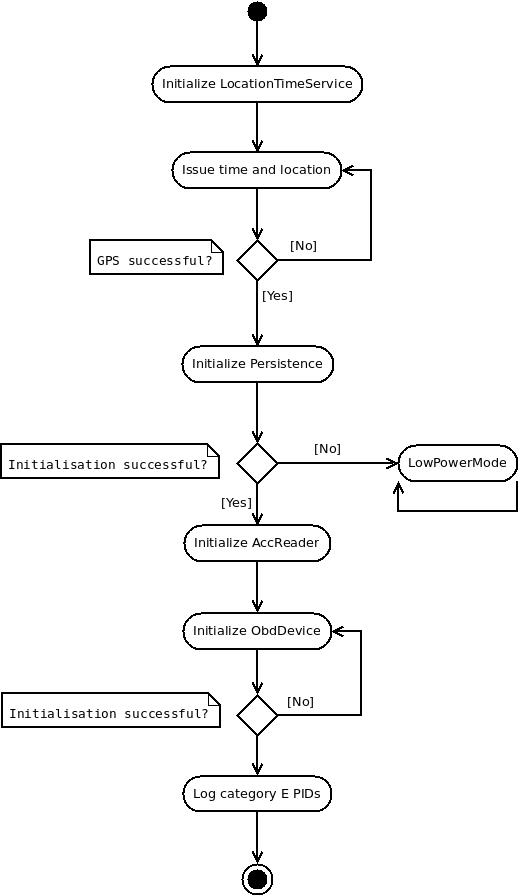
\includegraphics[width=\textwidth,height=20cm,keepaspectratio]{./img/Startup}
    \caption{Programmablauf der Initialisierung}
    \label{fig:setup}
  \end{center}
\end{figure}
\paragraph{}
Die Abbildung \ref{fig:setup} beschreibt den Ablauf des Programms beim Einstecken des Adapters in die Schnittstelle des Autos. Hervorzuheben ist, dass die Reihenfolge der Initialisierungen von großer Bedeutung ist. Während der Integration zeigte sich, dass die Persistenz-Klasse zur Initialisierung wesentlich mehr RAM benötigt als während des normalen Programmablaufs. Deshalb muss diese so früh wie möglich initialisiert werden. Nur die Klasse für GPS und Zeit muss zuvor bereit sein, da die Persistenzklasse diese während der Initialisierung aufruft.
\begin{figure}
  \begin{center}
    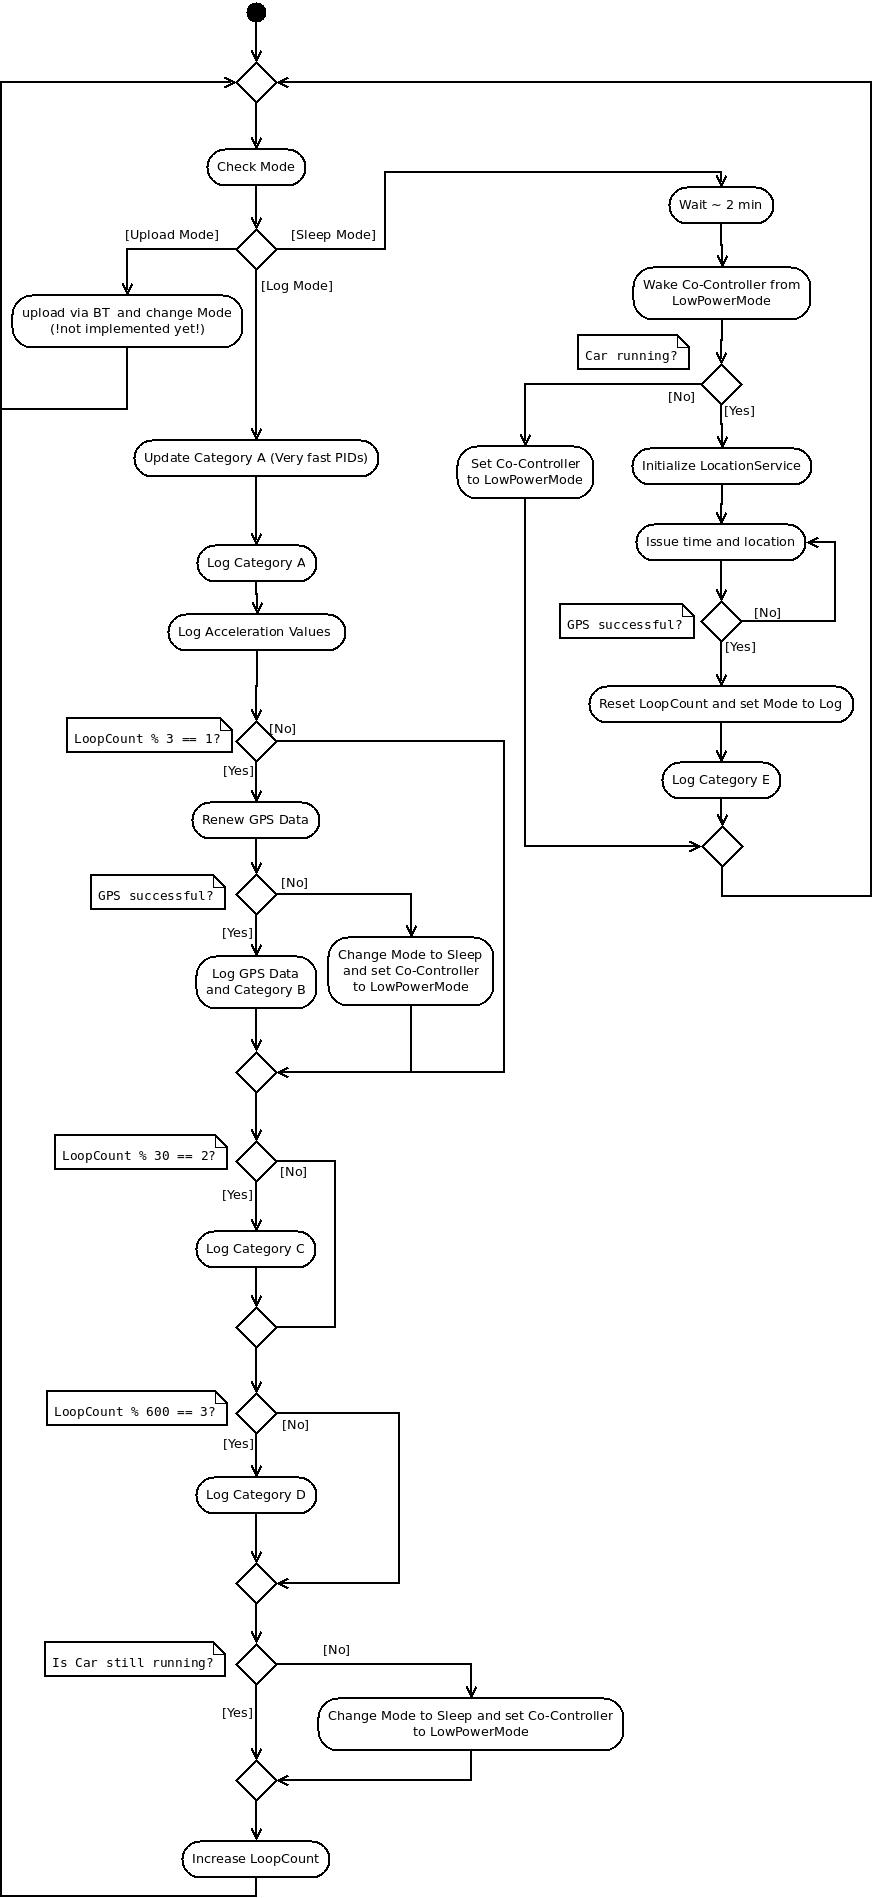
\includegraphics[width=\textwidth,height=20cm,keepaspectratio]{./img/ProgLoop}
    \caption{Programmablauf der Endlosschleife}
    \label{fig:loop}
  \end{center}
\end{figure}
In Abbildung \ref{fig:loop} ist der Ablauf des Programms ersichtlich, welches die eigentliche Funktionalität enthält. Dies wurde in drei Modi umgesetzt. Während des Logging-Modus werden die Fahrzeug-Daten gesammelt, auf eine SD-Karte geschrieben und per Bluetooth an ein Smartphone gesandt. Der Upload-Modus dient dazu, die gesammelten Daten auf der SD-Karte an die Smartphone-App weiterzugeben. Dies soll ein Entnehmen der Karte zum Auslesen der Daten optional machen. Der Schlafmodus dient letztendlich dazu, bei abgeschalteter Zündung das Bordnetz des Fahrzeugs möglichst wenig zu belasten.
\subsection{GPS-Empfänger}
Da ein zentrales Ziel der Applikation die Anfertigung eines Fahrtenbuches mit Streckenaufzeichnung ist, muss auch die Position des Fahrzeuges möglichst genau bestimmt werden. Der in diesem Projekt verwendete Freematics ONE bietet hier die Möglichkeit, einen externen GPS-Empfänger per UART anzubinden.
\paragraph{}
Um die Anschaffungskosten zu reduzieren, wurde zunächst untersucht, ob neben dem von Freematics verkauften GPS-Empfänger auch andere GPS-Receiver-Chips mit dem OBD-Dongle kompatibel sind.
Ein Problem bei dieser Untersuchung ist die Architektur des Freematics ONE, da die Kommunikation mit dem GPS-Empfänger nicht auf dem ATmega328p Haupt-Controller sondern auf einem STM32 Coprozessor ausgeführt wird. Leider ist der Code auf dem Coprozessor nicht öffentlich einsehbar und auch nicht ohne großen Aufwand auslesbar.
Ein weiteres Problem bestand darin, dass auch ein Öffnen des Gehäuses des von Freematics selbst vertriebenen GPS-Empfängers nicht zur Identifikation des Chips beitragen konnte. Es wurde allerdings klar, dass dieser nicht der Angabe auf der Produkthomepage des Freematics ONE entsprach. Der Empfänger-Chip ist nur mit einem QR-Code versehen und eine Recherche zum Hersteller verwies nur auf den chinesischen Produzenten des ganzen Empfänger-Moduls.(www.szgrltd.com)
\paragraph{}
Daher wurde eine andere Vorgehensweise zur Untersuchung der Kommunikation angewandt. Dazu wurde, wie in Abbildung \ref{fig:gpsAnalyse} abgebildet, ein zusätzlicher Arduino UNO als Zwischenstation in die UART-Kommunikation zwischen Dongle und Empfänger eingefügt. Zwei durch Software simulierte, serielle Schnittstellen auf dem Arduino UNO werden nun genutzt, um die vom Dongle und vom GPS-Empfänger gesendeten Daten aufzufangen, auf der über USB angeschlossenen seriellen Konsole eines Rechners auszugeben und an den jeweils anderen Kommunikationspartner weiterzuleiten.
\begin{figure}
  \begin{center}
    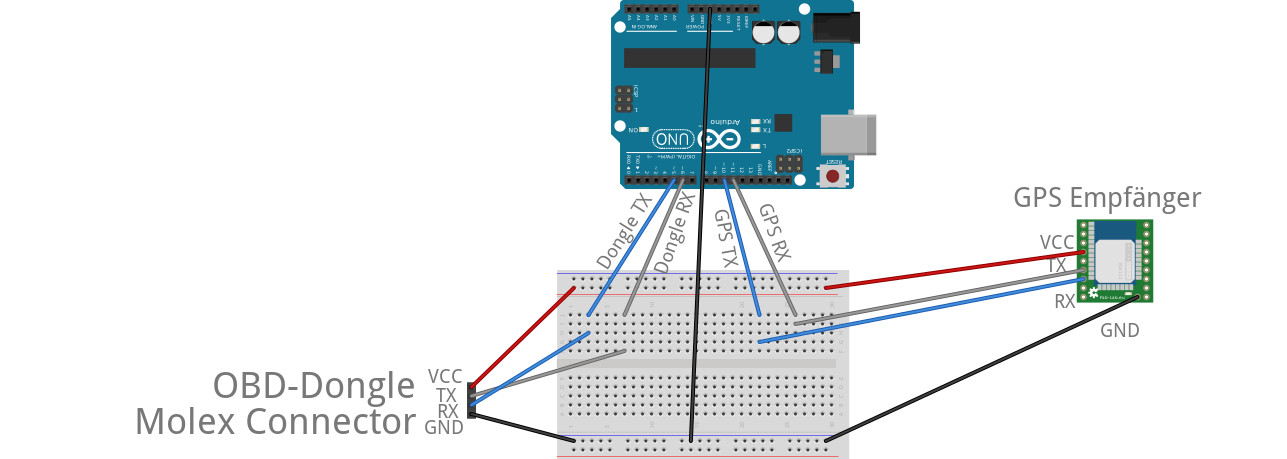
\includegraphics[width=\textwidth]{./img/gpsVersuch}
    \caption{Versuchsaufbau zur Analyse der UART-Kommunikation zwischen Dongle und GPS-Empfänger}
    \label{fig:gpsAnalyse}
  \end{center}
\end{figure}
\paragraph{}
Nach Auswertung der Kommunikation, stand fest, dass der von Freematics gelieferte Gps-Empfänger kompatibel zu einem u-blox UBX-G7020 ist. Dieser versendet standardmäßig Nachrichten gemäß dem NMEA Standard. Darüber hinaus wurde ersichtlich, dass der OBD-Dongle keine Nachrichten zum GPS-Chip sendet.
\paragraph{}
Da nun allerdings der konkrete Empfänger feststand, konnte dazu die entsprechende Protocol Specification heruntergeladen und mit weiteren GPS-Empfängern verglichen werden.
Letztendlich wurde ein Pixhawk GPS Empfänger für einen Modellbau-Quadrokopter auf Basis eines u-blox Neo6M mit zusätzlichem Magnetfeld-Sensor ausgewählt. Dieser Mikrochip verfügt zwar nicht über die exakt gleiche Protocol Specification, die ab Werk konfigurierte Kommunikation jedoch ist nahezu identisch und kompatibel mit der des von Freematics gelieferten Produktes.
\paragraph{}
Um den neuen Empfänger am Dongle zu betreiben, wurde an dessen Signal-Eingängen ein 2x2-Molex Stecker passend angelötet. Die I2C-Pins des Magnetfeld-Sensors wurden dabei nicht belegt.
\paragraph{}
Ein erster Test mit der mitgelieferten Software zeigte die grundsätzliche Funktion des neuen GPS-Moduls. Allerdings ist die Genauigkeit des Pixhawk-Empfängers etwas schlechter als die des UBX-G7020.

	\subsection{ \ac{OBD}-Schnittstelle}
		Da der Dongle vorwiegend genutzt werden soll um die \ac{OBD}-Daten (kurz \acp{PID}) aufzuzeichnen besitzt der Freematics ONE eine hierfür passende Schnittstelle. Bei den \acp{PID}\cite{OBD-2.net2018} handelt es sich um Daten die von bestimmten Sensoren (z.B. Drehzahl, Geschwindigkeit, Öl-Temperatur, ...) im Auto zu Verfügung gestellt werden.
		\ \\
		Bei \ac{OBD} handelt es sich um ein Protokoll welches nach dem \enquote{challenge-response} funktioniert. Dabei werden vom Client (Dongle) anfragen an den Server (\ac{OBD}-Steuergerät im Auto) gesendet. Dieses antwortet anschließend mit den Werten des entsprechenden Sensors.
		\ \\
		Da es Abhängig vom vorliegenden Auto abhängig ist, welche Steuergeräte verbaut sind und was somit für \acp{PID} unterstützt werden, ist es nicht bei jedem Auto möglich die selben Daten auszulesen.
		\ \\
		Da weiterhin der Platz auf dem Freematics ONE (sowohl RAM als auch Flash) sehr begrenzt ist, wurde von vorne herein entschieden, nur bestimmte \acp{PID} zu verwenden. Insgesamt wurden xy viele \acp{PID} ausgewählt. Um sowohl die \ac{OBD}-Schnittstelle als auch den Prozessor im Freeatics ONE unter wenig Last auszusetzen, dabei allerdings möglichst viel Nutzen aus den gewonnen Informationen ziehen zu können, wurden die \acp{PID} in unterschiedliche Gruppen eingeteilt. 
		\ \\
		Eine Gruppe entspricht somit einem Zusammenschluss aus \acp{PID} welche alle in einem gleichen Zeitintervall abgerufen werden. Es wurde sich für folgende Gruppen entschieden (Tabelle \ref{KategorieTable}):
		
		\begin{center}
			\begin{tabular}{|c|c|}
				\hline 
				Kategorie & Intervall \\ 
				\hline 
				A & 500ms \\ 
				\hline 
				B & 1,5s \\ 
				\hline 
				C & 15s \\ 
				\hline 
				D & 5min \\ 
				\hline 
				E & neue Route \\ 
				\hline 
				F & neues Auto \\ 
				\hline 
			\end{tabular} 
			\label{KategorieTable}		
		\end{center}

		
		Der Tabelle xyc kann zum einen entnommen werden, welche \acp{PID} ausgewählt wurden und in welcher Kategorie sie zugeordnet wurde.
		
		\begin{center}
			\begin{tabular}{|c|c|c|}
				\hline 
				Name & Wert & Kategorie \\ 
				\hline 
				Engine coolant temperature & 0x5 & C \\ 
				\hline 
				Engine RPM & 0x0C & A \\ 
				\hline 
				Vehicle speed & 0x0D & A \\ 
				\hline 
				Run time since engine start & 0x1F & C \\ 
				\hline 
				Distance traveled with malfunction indicator lamp & 0x21 & D \\ 
				\hline 
				Fuel tank level input & 0x2F & D \\ 
				\hline 
				Absolute barometric pressure & 0x33 & C \\ 
				\hline 
				Ambient ari temperature & 0x46 & C \\ 
				\hline 
				Fuel type & 0x51 & E \\ 
				\hline 
				Ethanol fuel \% & 0x52 & E \\ 
				\hline 
				Relative accelerator pedal position & 0x5A & A \\ 
				\hline 
				Engine oil temperature & 0x5C & C \\ 
				\hline 
				Engine fuel rate & 0x5E & A \\ 
				\hline 
				Driver's demand engine-percent torque & 0x61 & A \\ 
				\hline 
				Actual engine-percent torque & 0x62 & A \\ 
				\hline 
				Engine reference torque & 0x63 & A \\ 
				\hline 
				Engine run time & 0x7F & C \\ 
				\hline 
			\end{tabular} 
		\end{center}
		
		
		
	
	
	
	
	
	


\subsection{Zeit}
Wie bereits erwähnt, muss auch auf dem Dongle eine Repräsentation der genormten Zeit vorhanden sein. Zunächst soll jeder erfasste Datenwert mit einem Zeitstempel versehen werden um mit einer totalen Ordnung die Analyse dieser Werte erst zu ermöglichen. Zum anderen sollen die Datenwerte mit einem Intervall von 200 Millisekunden erfasst werden.
\paragraph{}
Die Anforderung nach einem genauen Zeitintervall von 200 Millisekunden zwischen dem Abrufen der OBD-Werte der Klasse A kann durch den Einsatz eines Hardware-Timers und Interrupts gelöst werden.
Auf dem ATmega328p Hauptcontroller stehen dem Entwickler 3 Hardware-Timer zur Verfügung. Allerdings muss hierbei beachtet werden, dass die Arduino-Bibliothek den Timer 0 für die Funktionen delay() und millis() verwendet und diese daher unangetastet bleiben sollten.\cite{arduinoTimer}
Da die Intervalle zum Abrufen der PID-Klassen B, C und D ein Vielfaches der 200 Millisekunden der Klasse A sind, müssen für diese keine weiteren Timer verwendet werden. Statt dessen kann ein einfacher Vergleich in Kombination mit dem Modulo-Operator genutzt werden (vgl. Abbildung \ref{fig:loop}).
\subsection{Beschleunigungssensor}
Zunächst wurde ermittelt, welcher Sensor im Dongle verbaut wurde. Anhand der Informationen auf der Produkthomepage sowie des Source-Codes des Treibers wurde ersichtlich, dass ein MPU-9250 MEMS Bewegungssensor mit jeweils 3 Achsen für Beschleunigungs-, Drehraten- und Magnetfeldmessung verbaut ist. Hierbei ist besonders, dass der Sensor für das Magnetfeld als I²C-Submodul am Sensor ausgeführt ist.

\chapter{Implementierung}
\label{sec:implementation}

Im folgenden Kapitel wird zunächst ein Überblick über die Implementierung der App, des Backends und des Dongels gegeben. Hierbei wird auf spezielle Anforderungen bzw. Lösungsideen eingegangen. \todo{irgendwas musss hier stehen... sonst schauts komisch aus}

\section{App}

\subsection{Sichten}

\subsubsection{Visualisierung}
\label{sec:appSichtAnzeige}

\begin{wrapfigure}[16]{r}{0.5\textwidth}
  \begin{center}
	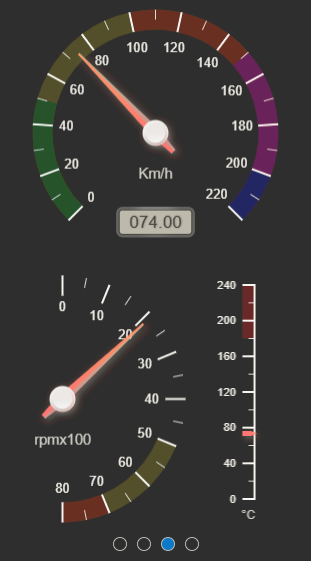
\includegraphics[width=0.3\textwidth]{./img/App_Speedo}
	\caption{Ansicht \enquote{Speedo}}
	\label{fig:App_Speedo}
  \end{center}
\end{wrapfigure}

In der Smartphone-App stehen mehrere Sichten für die Anzeige der Live Daten zur Verfügung. Diese können über eine Callback-Funktion auf schon vorbereite Daten vom Dongle und Smartphone zugreifen. Dadurch müssen sich diese nur noch um die bloße Darstellung der Daten kümmern. Jede Sicht fügt sich dabei selbst der Liste der Views hinzu und wird dadurch in der App angezeigt. So ist es ein Leichtes, sobald neue Daten vom Dongle zur Verfügung stehen sollten, fast unbegrenzt weitere Ansichten hinzuzufügen.
\\
Zurzeit stehen drei Sichten zur Auswahl. Eine einfache Liste mit allen vom Dongle und Smartphone verfügbaren Werten. Darunter die Geschwindigkeit, gemessen vom Dongle sowohl als auch vom Handy, Drehzahl, Kühlwassertemperatur und die GPS Daten des Dongles und Smartphones.
\\
Des weiteren eine Tachoansicht (siehe Abbildung \ref{fig:App_Speedo}), welche die momentan gefahrene Geschwindigkeit, Drehzahl und die Kühlwassertemperatur anzeigt.
\\
Die letzte zurzeit implementierte Sicht ist ein Vergleich der gemessenen Geschwindigkeit von der OBD-Schnittstelle und der ermittelten Geschwindigkeit vom GPS-Sensor. Diese sind jeweils als Tacho visualisiert.

\subsubsection{Konfiguration}
\label{sec:appSichtKonfiguration}

Die \enquote{Konfiguration View} (siehe Abbildung \ref{fig:APP_Configuration}a) ist eine spezielle Sicht, in der unter anderem die Verbindung zum Dongle hergestellt werden kann. Dazu steht ein Dialog (siehe Abbildung \ref{fig:APP_Configuration}b) zum Suchen aller in der Umgebung befindlichen Bluetooth-Geräte zur Verfügung. Beim Anklicken wird versucht eine Verbindung zu diesem Device aufzubauen. Durch Klicken auf den Button \enquote{Test} kann geprüft werden, ob zurzeit eine Verbindung zu diesem besteht. Das gleiche Prinzip ist auch für die Verbindung zum Backend vorhanden. Hier öffnet sich beim Button \enquote{Connect} eine Liste der Verbindungsparameter, die dazu benötigt werden. Außerdem sind in dieser Sicht noch die App-Einstellungen (z.B Km/H oder Mp/H) änderbar und die Logging-Liste auslesbar.

\begin{figure}[H]
	\centering
	\subfigure[Übersicht]{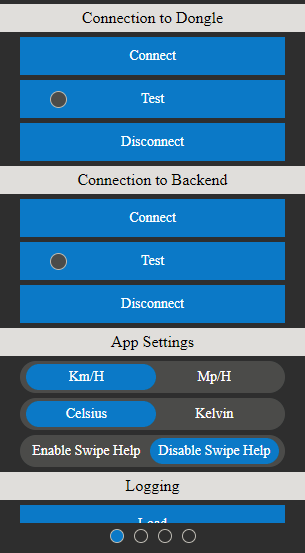
\includegraphics[width=0.3\textwidth]{./img/APP_Configuration}}
    \label{fig:APP_Configuration_View}
    \hspace{1cm}
	\subfigure[Dialog \enquote{Dongle - Connect}]{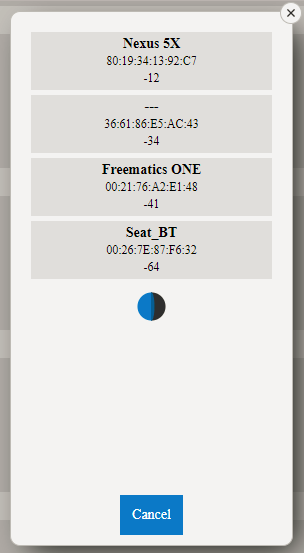
\includegraphics[width=0.3\textwidth]{./img/App_Bluetooth_Search}}
	\label{fig:App_Bluetooth_Search}
	\caption{Ansicht \enquote{Konfiguration}}
	\label{fig:APP_Configuration}
\end{figure}

\subsection{Bluetooth}
\label{sec:appBluetooth}

Die Kommunikation mit dem Dongle erfolgt über Bluetooth Low Energy. Dafür wurde in der App das Cordova-Plugin \enquote{ble-central} verwendet. Das Plugin dient als einfacher \enquote{Wrapper} zu den nativen Funktionen. Außerdem mussten spezielle BLE-Konventionen eingehaltet werden. So können Daten nur durch das Abonnieren vom Sender angebotener \enquote{Characteristic}s (32 Bit ID) von \enquote{Service}s (32 Bit ID) empfangen und gesendet werden. Welche \enquote{Service}s und \enquote{Characteristic}s angeboten werden, müssen vorher angefragt  werden. Hierbei gibt es zum einen Standard-Services (z.B. Device Information - 0x180A) und zum anderen Custom-Services zum Übertragen von speziellen Daten. Das Bluetooth Modul vom Dongle ist nicht veränderbar und sendet alle Daten, die über die serielle Konsole gesendet werden über den Service 0xFFE0 und der Characteristic 0xFFE1. Dadurch kann das für BLE empfohlene Schema, das Trennen der Daten durch andere Characteristic-ID, nicht angewandt werden. Somit muss für die unterschiedlichen Anforderungen weitere Merkmale zur Unterscheidung der Daten eingebaut werden.\cite{BluetoothLowEnergy}
\\
Wie auch bei normalen TCP-Netzwerkkommunikation können bei Bluetooth die Daten in Pakete aufgeteilt werden. In diesem Fall müssen die Daten beim Empfangen wieder zusammengesetzt werden. Falls in einem Callback festgestellt wird, dass ein Datensatz nicht vollständig angekommen ist, wird dieser Teil vom Puffer des aktuellen Callback's entfernt und dem Zukünftigen am Anfang hinzugefügt.

\subsection{GPS}
\label{sec:appGPS}

Um einen Vergleich der Genauigkeit des GPS-Sensors im Dongle zu erhalten, wird dieser mit dem GPS-Sensor des Smartphones verglichen. Dazu wird entweder die letzte gespeicherte Position des Betriebssystems genutzt, falls diese nicht länger als 10 Sekunden alt ist, oder eine neue Position angefordert.

\subsection{Zugriff auf Identity Server}

Um mit den Backend kommunizieren zu können, muss zuerst die Authentifizierung über den Identity Server stattfinden. Dieser bietet dafür mehrere Möglichkeiten (z.B. Authorization Code, Client Credentials). In der App wird die Authentifizierungsmethode \enquote{Password Grand} verwendet. Dabei wird ein JSON-Objekt (siehe nachfolgenden Code) über einen HTTP-Request, mit Hilfe von AJAX, an den Server gesendet. Das Objekt enthält den Namen und das Passwort des Benutzers, sowie eine Client ID, die extra für die APP ausgestellt wurde, und ein dazu passendes Geheimnis. Der Authentifizierungsserver liefert nun ein Token zurück, mit dem nun mit dem Backend für eine gewisse Zeit kommuniziert werden kann. Dieses wird dem Backend bei jedem Request über dem HTTP Header mitgesendet. \cite{RFC6749}\cite{RFC6750}

\noindent
\begin{minipage}{\linewidth}
\begin{lstlisting}
{
	username: Store.get(username),
	password: Store.get(password),
	scope: "openid",
	grant_type: "password",
	client_id: Settings.Backend.clientId,
	client_secret: Settings.Backend.secret
}
\end{lstlisting}
\end{minipage}

\subsection{Konfiguration}
\label{sec:appKonfiguration}

Es gibt Grundlegend drei Arten von Konfigurationswerten. Zum einen statische, Standard- und Initial- Werte (z.B Timeouts, Client ID / Secret, Standard Ansicht), die fest im Code integriert sind. Diese sind zur besseren Wartbarkeit in der Datei \enquote{Settings} als JSON-Objekt gesammelt. Veränderbare Einstellungen können entweder im \enquote{Local Store} oder im \enquote{Session Store} als Key-Value-Paar angelegt werden. Dabei sind sie entweder flüchtig (z.B. für den Token), damit zeitlich begrenzt gelöscht, oder fest (z.B. für die Sprache) gespeichert.

\subsection{Mehrsprachigkeit}
\label{sec:appMehrsprachigkeit}

Um die geforderte Mehrsprachigkeit zu gewährleisten, sind alle verwendeten Texte in einer JSON-Datei zusammengefasst. In dieser sind die Texte als Key-Value-Paar abgespeichert (z.B. load: „load“); falls der beinhaltende Text eine Übersetzung benötigt, kann das Key-Value-Paar optional in die jeweiligen Sprachen aufgeteilt werden (z.B.
load: \{ en: „load“, de: „laden“ \}). Die \enquote{String}-Klasse ermittelt dann mit Hilfe der eingestellten Sprache den zu verwendenden Text. Falls der Text in der aktuellen Sprache nicht verfügbar ist, wird die Standardsprache (Englisch) zurückgegeben.

\pagebreak

\subsection{Weitere Anzeigeelemente}
\label{sec:appAnzeigeelemente}

\begin{wrapfigure}{R}{0.45\textwidth}
  \begin{center}
	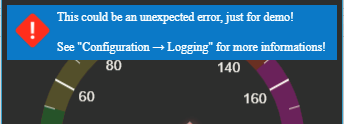
\includegraphics[width=0.4\textwidth]{./img/App_ErrorPanel}
	\caption{Error Panel}
	\label{fig:App_ErrorPanel}
	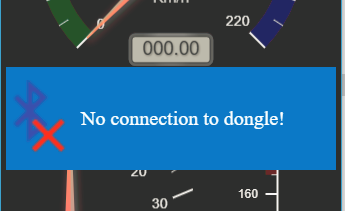
\includegraphics[width=0.4\textwidth]{./img/App_NoConnectionPanel}
	\caption{No Connection Panel}
	\label{fig:App_NoConnectionPanel}
    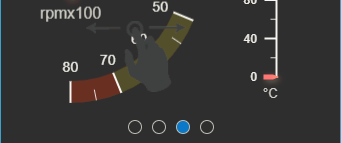
\includegraphics[width=0.4\textwidth]{./img/App_SwipeHelp}
    \caption{Swipe Help}
    \label{fig:App_SwipeHelp}
    
\includegraphics[width=0.4\textwidth]{./img/App_ViewCircles}
    \caption{View Circles}
    \label{fig:App_ViewCircles}
    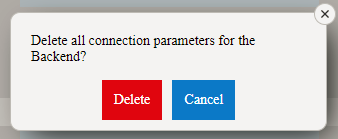
\includegraphics[width=0.4\textwidth]{./img/App_Dialog}
    \caption{Dialog}
    \label{fig:App_Dialog}
  \end{center}
\end{wrapfigure}

Für das Anzeigen von speziellen Informationen gibt es mehrere Elemente. Zur Mitteilung von unerwarteten Fehlern gibt es einen Fehler Dialog (siehe Abbildung \ref{fig:App_ErrorPanel}). Dieser zeigt am oberen Rand des Bildschirmes eine Kurzinformation zum Fehler und die Information, dass sie im Logging-Bereich der Konfigurationsansicht komplett eingesehen werden kann an.
\\
Falls keine Bluetooth Verbindung zum Dongle besteht oder diese abgebrochen oder gestört ist, wird im mittleren Teil des Displays ein Panel (siehe Abbildung \ref{fig:App_NoConnectionPanel}) angezeigt, das dieses Ereignis visualisiert.
\\
Für die erste Benutzung der App wird beim Starten der App eine bewegende Anzeige (siehe Abbildung \ref{fig:App_SwipeHelp}) eingeblendet, die den Anwender signalisieren soll, dass durch nach Links und Rechts wischen weitere Ansichten und Optionen zur Verfügung stehen. Diese Funktion kann, falls sie als Störend empfunden wird, in der Konfigurationssicht deaktiviert werden.
\\
Um den Benutzer über die gerade angezeigt Sicht zu informieren, sind am unteren Ende der App Kreise (siehe Abbildung \ref{fig:App_ViewCircles}) für jede View symbolisiert. Der Kreis für die zurzeit sichtbare Ansicht ist dabei ausgefüllt.
\\
Für manche Funktionen bieten sich Dialoge am besten an. Hier gibt es zum einen kleine Dialoge wie in Abbildung \ref{fig:App_ViewCircles} zu sehen und zum anderen Fullscreen-Dialoge, für zum Beispiel das Suchen der aktuellen Bluetooth Geräte im Umkreis (siehe Kapitel \ref{sec:appSichtKonfiguration}).







\section{Backend}
Als Technologie für die Implementierung des Backends wird das Asp.Net Core Framework von Microsoft eingesetzt. Grund dafür ist, dass alle benötigten Funktionen wie Webfrontends, REST APIs oder Identity Management nativ und gleichzeitig plattformunabhängig unterstützt werden. Als Programmiersprache wird C\# eingesetzt.

\subsection{Authentifizierung und Autorisierung}
Für die Umsetzung der Benutzerauthentifizierung und die Rechteverwaltung wird IdentityServer4\cite{Allen2016} eingesetzt. Dieses Framework erlaubt eine moderne zentralisierte Identitätsverwaltung für verschiedene Anwendungsszenarien basierend auf OpenId und OAuth2. 

\begin{figure}[h]
  \begin{center}
    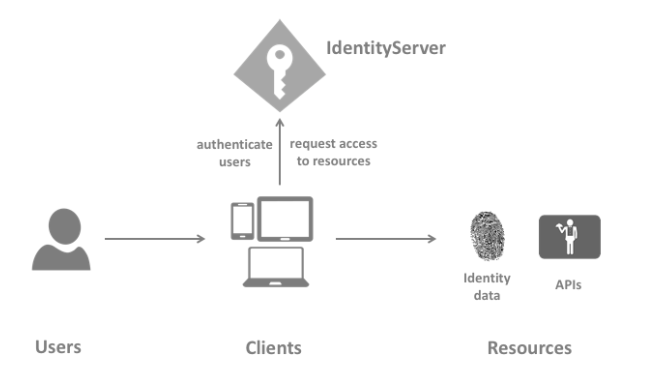
\includegraphics[width=\textwidth]{./img/BackendIdentityServer.png}
    \caption{Terminologien des Identity Servers}
    \label{fig:backendIdentityServer}
  \end{center}
\end{figure}

Das Grundkonzept des Identity Servers wird in Abbildung \ref{fig:backendIdentityServer} gezeigt. \textbf{Benutzer} greifen dabei über verschiedene \textbf{Clients} auf geschützte \textbf{Ressourcen} wie APIs oder Anwendungsbereiche zu, die von dem Identitätsserver geschützt werden. Dieses Konzept passt auf das in diesem Projekt entstehende Szenario, in dem Benutzer entweder über die Smartphone App oder das Webfrontend des Backends (Clients) auf die Web API zugreifen (Ressource).

\begin{figure}[h]
  \begin{center}
    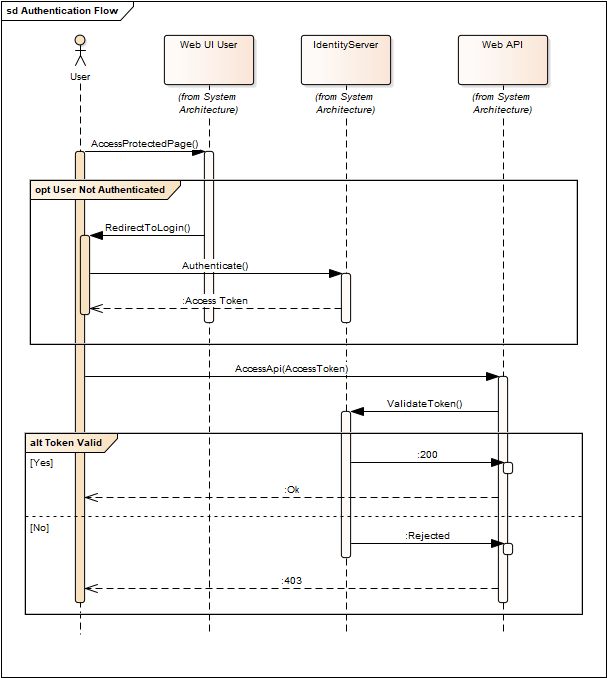
\includegraphics[width=\textwidth]{./img/BackendAuthenticationFlow.png}
    \caption{Ablauf der Authentifizierung beim Zugriff auf geschützte Ressourcen}
    \label{fig:backendAuthenticationFlow}
  \end{center}
\end{figure}

Der implementierte Ablauf der Authentifizierung erfolgt nach dem in Abbildung \ref{fig:backendAuthenticationFlow} skizzierten Schema. Beim Zugriff auf eine geschützte Funktion im Web UI wird der Benutzer auf die Login Seite des Identity Servers weitergeleitet, wo er sich entweder registrieren oder einloggen kann. Nach erfolgreicher Authentifizierung generiert der Identity Server ein Access Token, welches in der Session des Benutzers gespeichert wird und Informationen über den Benutzer, die für ihn freigegebenen Ressourcen sowie die dem Nutzer zugeordneten Claims enthält. Bei einem anschließenden Zugriff die Web API wird dieses Token mitgeschickt und von der API beim Identity Server validiert.

\subsection{Datenbank und Zugriff}
\label{sec:dataAccess}
Als Datenbank wird MySql eingesetzt da es einfach in der Anwendung und schlank im Betrieb ist. Als alternative wurde ebenfalls Sql Server evaluiert, was den Vorteil der besseren Integration in die Asp.Net Core Umgebung gehabt hätte. Der zugehörige Docker Container (vgl. \ref{sec:backendDeployment}) hat jedoch 4GB Arbeitsspeicher erfordert, was zusätzlich zum normalen Betriebssystem und der Entwicklungsumgebung mehr als die momentan üblicherweise verbauten 8GB \ac{RAM} übertrifft.\todo{Weshalb es auf unseren Systemen nicht getestet werden konnte - vllt ergänzen}

Der Zugriff auf die Datenbank erfolgt nicht direkt über SQL-Anfragen sondern über Entity Framework, ein Framework für objektrelationale Abbildung. Dabei werden die Daten im Hintergrund in Collections geladen, sodass es für den Benutzer aussieht, als würden die Daten direkt im RAM liegen. Dieses System bietet - insbesondere in Kombination mit \ac{LINQ} in C\#- den Vorteil, dass der Code wesentlich übersichtlicher und leichter verständlich wird, da das direkte Laden der Daten mittels SQL-Anfragen und anschließendem manuellen Einlesen entfällt.

Für die Integration von Entity Framework für MySql Datenbanken in einer Asp.Net Core Umgebung muss ein Third Party NuGet Paket\cite{Microsoft2018} verwendet werden, da zum Zeitpunkt der Entwicklung keine native Anbindung zur Verfügung steht. Das verwendete Paket hat allerdings Performanceprobleme bei der Verarbeitung größerer Datenmengen. Schon das Speichern und Laden von Fahrten mit einer Rohdatenmenge von ~500kB führen zu Verzögerungen von ca. 30 Sekunden. Die einzig verbleibende Alternative um das Problem zu beheben ist der Austausch der Datenbank, wozu während der Projektlaufzeit keine Ressourcen mehr zur Verfügung stehen.

\subsection{Bereitstellung}
\label{sec:backendDeployment}
Da das Backend aus verschiedenen zunächst unabhängigen Komponenten besteht und einige Voraussetzungen bezüglich der Infrastruktur mit sich bringt, ist die Bereitstellung einer Produktivumgebung nicht trivial. 
Aus diesem Grund wird die Containervirtualisierung Docker eingesetzt, um das Gesamtsystem leicht installierbar zu machen.

Docker\cite{Inc.2018} unterscheidet von normalen virtuellen Maschinen darin, dass nicht für jede Instanz ein gesamtes Hostsystem emuliert wird, sonder lediglich die Applikation samt ihrer Abhängigkeiten in dem Container stecken. In der Terminologie wird bei Docker zwischen Containern und Images unterschieden. Ein Image ist dabei ein Speicherabbild, aus dem heraus sich mehrere Container starten lassen (vergleichbar mit Klassen und Instanzen bei objektorientierter Programmierung). Für die Installation bedeutet das, dass nur die Images aller am System beteiligten Module zur Verfügung stehen müssen um aus jedem Image einen Container zu starten. Um das hochfahren komplexerer Anwendungen, die aus mehreren Containern bestehen, zu erleichtern, gibt es das Tool Docker Compose. Hiermit lassen sich verschiedene Parameter einstellen und alle Container gemeinsam starten was den Aufwand bei der Bereitstellung weiter reduziert. 

Um das SmartCar Backend in einer neuen Umgebung auszurollen werden lediglich die Images der Module, sowie das docker-compose File benötigt. Zusätzlich muss natürlich Docker auf dem Zielsystem installiert sein. Ist alles vorhanden, lässt sich über den Befehl \texttt{docker-compose up} die gesamte Umgebung ohne zusätzliche Installationen hochfahren.

\subsection{Datenanalyse am Beispiel Kraftstoffverbrauch}
Wie bei \ref{Sec_AnayseDerAufgezeichnetenDaten} beschrieben ist, war es von Anfang an ein Ziel die Daten nicht nur zu sammeln, sondern auf diesen anschließend Analysen auszuführen um dem Fahrer somit einen Zugewinn an Informationen zu ermöglichen. 

Eine dieser Analysen ist die Ermittlung des Kraftstoffverbrauchs. Aktuelle Autos stellen diese Information dem Fahrer inzwischen zwar meist per Bordcomputer zur Verfügung. Fahrer älterer Fahrzeuge erhalten diese Informationen jedoch nicht. Weiterhin könnte bei der Berücksichtigung des \enquote{Dieselskandals} aus jüngster Zeit auch die Frage aufkommen, ob die angezeigten Informationen überhaupt der Realität entsprechen, da ja bereits die Herstellerangaben im täglichen Betrieb äußerst selten eingehalten werden können.

Um eine solche Analyse durchführen zu können, müssen zuerst die benötigten Informationen aus dem Track extrahiert werden:\newline
Da die Anbindung der Datenbank (siehe \ref{sec:dataAccess} Absatz 3) das \enquote{Bottelneck} des Backends darstellt, wurde um dieses möglichst wenig zu belasten keine generischen Funktionen geschrieben um die zur Berechnung benötigten Daten aus den Traces extrahieren, sondern für jede Analyse eine eigene. In diesen werden die Daten eines Traces durchlaufen und bei Übereinstimmung der \acs{PID} mit den ausgewählten \acp{PID} extrahiert.

Für aktuelle Autos ist es mit den gemessenen Verbrauchswerten anschließend möglich einen Kraftstoffverbrauch zu bestimmen bzw. diesen gegenüber z.B. der Geschwindigkeit in einem Diagramm anzuzeigen.

Bei älteren Autos, welche nicht messen wie viel Kraftstoff verbraucht wird oder diese Informationen nicht über \ac{OBD} zu Verfügung stellen ist die Analyse komplexer. Aus diesem Grund gibt es auch mehrere wissenschaftliche Arbeiten die sich in diesem Zusammenhang auch mit der \ac{OBD} Schnittstelle beschäftigen \cite{obdConsumption} \cite{rtFuel}. Der Konsens dieser Arbeiten ist, dass sich der Momentanverbrauch, sofern er sich nicht über die \ac{PID} 0x5E auslesen lässt, mithilfe anderer Datenwerte Berechnen lässt.
Dazu wird im Grunde die Formel \ref{GrundFormelMomentanVerbrauch} verwendet. 

Hier gibt die Konstante $AirFuelRatio_\text{Stöch}$ das Verhältnis von Luft und Kraftstoff an, bei der alle
Kohlenwasserstoff-Moleküle mit allen Sauerstoffmolekülen der angesaugten Luft reagieren. Dieses
Verhältnis ist für den Verbrennungsvorgang optimal, und beträgt bei Ottomotoren 14,7 und bei
Dieselmotoren 14,5.

\begin{equation}
\label{GrundFormelMomentanVerbrauch}
Sprit(\frac{g}{sec}) = \frac{Luftmasse(\frac{g}{sec})}{\lambda*AirFuelRatio_\text{Stöch}}
\end{equation}

Ausgehend von Formel \ref{GrundFormelMomentanVerbrauch} kann nun anhand der Dichte auf den Momentanverbrauch in Litern geschlossen werden. Dazu verwendet man Formel \ref{DichteZuVerbrauchInLiter}. Dabei ist $\rho$ die gemittelte Dichte des Kraftstoffs. Für Ottokraftstoff beträgt diese etwa 747,5
Gramm pro Liter, für Diesel dagegen etwa 832,5 Gramm pro Liter\cite{Aral2018}. 

\begin{equation}
\label{DichteZuVerbrauchInLiter}
Sprit(\frac{l}{sec}) = \frac{Sprit(\frac{g}{sec})}{\rho}
\end{equation}
 
Für die Berechnung wird als nächstes $\lambda$ benötigt. Hierbei handelt es sich um das gemessene Luft-Treibstoff-Verhältnis, welches über eine Lambda-Sonde gemessen wurde. Dieser Wert kann laut ISO 15031-5 mit Formel \ref{FormelFuerLambda} berechnet werden.

\begin{equation}
\label{FormelFuerLambda}
EQRAT 11_\text{PID 24}=DATAab_{(\text{PID 24})}*(\frac{DATAa_{(\text{PID 4F})}}{65535})
\end{equation}

$DATAab_{\text{PID 24}}$ entspricht hierbei dem Sensorwert, welcher über die ersten beiden Bytes der \ac{PID} 0x24 ausgelesen wird (alternativ können je nach Verfügbarkeit auch die \acp{PID}) 0x25-0x2B oder 0x34-0x3B verwendet werden).
\newline
$DATAa_{(\text{PID 4F})}$ gibt die Skalierung an.
\newline
Sollten die \acp{PID}) 0x24-0x2B oder 0x34-0x3B nicht verfügbar sein, gibt es auch hierfür weitere Möglichkeiten zur Berechnung. Diese benötigen jedoch immer spezifischere Daten für das Verwendete Auto und wurden deshalb mangelns fehlender Messtechnik zur Überprüfung auf Korrektheit nicht weiter implementiert.

Als Letztes wird für die Berechnung noch der Luftfluss benötigt. Dieser lässt sich im einfachsten Fall mithilfe der \ac{PID} 0x10 ermitteln und anschließend durch den zugehörigen Korrekturfaktor \ac{PID} 0x50 korrigieren.

Für den Fall, dass der Wert des Luftmassesensors nicht abrufbar ist, so wurde in \cite{obdConsumption} eine Möglichkeit vorgestellt, wie sich dieser Wert mithilfe der Werte der EngineLoad (\ac{PID} 0x04) und der Motordrehzahl (\ac{PID} 0x0C0) ermitteln lässt. Jedoch werden auch für diese Berechnung Fahrzeug-spezifische Messdaten benötigt welche meist nicht vorliegen.

 
 
 
 

\section{Dongle}

\subsection{GPS und Zeit} 
\label{ImplGpsUndZeit}
Um den GPS-Empfänger auch in der in diesem Projekt geschriebenen Dongle-Software zu nutzen, wurde zunächst der Code des von Freematics veröffentlichten Treibers für den Coprozessor übernommen, da dieser den Datenaustausch mit dem Empfänger regelt und die serielle Schnittstelle mit diesem verbunden ist. Um die Kommunikation von der eigentlichen Anwendungslogik abzutrennen, wurde eine weitere LocationTimeService-Klasse auf Ebene der Intermediate-Layer implementiert. Diese bietet nun vereinfachten Zugriff auf die gemessenen Werte des geografischen Längen- und Breitengrads, der Höhe über Normalnull und die Anzahl der verfügbaren Satteliten. Darüber hinaus stellt sie auch Funktionen zum erneuten Abrufen und Speichern der GPS-Daten und zur Initialisierung der Kommunikation mit dem GPS-Chip über UART zur Verfügung. Dabei ist zu beachten, dass die Anzahl der Satelliten für eine möglichst korrekte Positionsbestimmung zwischen 4 und 14 liegen muss \cite{gpsPrecision}.

Während der Initialisierung des LocationService, wird bis zu fünf mal versucht, über den Treiber des Coprozessors eine serielle Datenübertragung aufzubauen. Um die Genauigkeit vor allem des Pixhawk-Empfängers zu verbessern, wird während der Initialisierung der LocationService-Klasse der Intermediate Schicht der GPS-Chip für die Nutzung für \ac{SBAS} konfiguriert. Dazu wird die write-Methode des Treibers genutzt, mit dem ein Byte-Array 1:1 übertragen werden kann.
Gemäß der Protocol-Specification beider GPS-Module, kann SBAS mit folgendem Code konfiguriert werden:
\begin{lstlisting}
  uint8_t cmd[] = {0xB5, 0x62, 0x06, 0x16, 0x00, 0x08, 0x03, 0x07, 0x00, 0x00, 0x00, 0x00, 0x51, 0x7F, 0xEE };
  uint8_t cmdLen = 15;
  [...]
  //send config command
  _coProc->setTarget(TARGET_GPS);
  _coProc->write(cmd, cmdLen);
\end{lstlisting}

Um die Kommunikation mit dem Coprozessor nicht unnötig zu belasten und die Verarbeitung der OBD-Daten auf diesem nicht zu kompromittieren, werden die Sensordaten nur nach Bedarf mit der Methode RenewGPSData in Member-Variablen der LocationTimeService-Klasse zwischengespeichert. Ein Aufruf der Getter-Methoden führt nur dazu, dass diese zwischengespeicherten Werte ausgegeben werden.
\paragraph{}
Da mit dem GPS auch Zeitinformationen übertragen werden, werden diese genutzt, um die aktuelle Zeit auf dem System verfügbar zu machen. Dazu erhält die LocationTimeService-Klasse zusätzliche Methoden um die Hardware-Timer 1 und 2 zu konfigurieren und um die Millisekunden seit dem 1.1.1970 abzurufen. Diese Zeit wird in der LocationTimeService-Klasse als Membervariable zwischengespeichert.
\paragraph{}
Um die GPS-Information zur \enquote{Unix-Epoch} umzuwandeln wird auf Funktionen der Header-Datei \enquote{time.h} zurückgegriffen, welche in der Arduino Header Sammlung enthalten ist. Allerdings muss während der Konversion der Wert 946684800 hinzuaddiert werden, da Arduino die Epoch seit dem 1.1.2000 rechnet und der genannte Wert den Sekunden zwischen 1.1.1970 und 1.1.2000 entspricht. Bei der Rückgabe der Millisekunden muss darauf geachtet werden, dass ein Datentyp mit 64 Bit verwendet wird und auch keine impliziten Umwandlungen bei der Berechnung auftreten.
\paragraph{}
In diesem Zuge wird Timer 1 mit global sichtbaren Funktionen und einem Interrupt so konfiguriert, um das Logging-Intervall von 500 ms einzuhalten. Timer 2 wird ähnlich konfiguriert, sorgt aber dafür, dass der zwischengespeicherte Epoch-Wert alle 8 Millisekunden um diesen Wert erhöht wird. Dadurch muss nicht jedes mal die GPS-Zeit abgerufen werden, wenn der Zeitstempel benötigt wird.

\subsection{ \ac{OBD}-Schnittstelle}
	Da die Kommunikation mit der \ac{OBD}-Schnittstelle ebenfalls über den Coprozessor abgewickelt wird, von welchem die Software nicht bekannt ist, wurde hier die von Freematics bereitgestellte Klasse \enquote{COBDSPI} verwendet. Diese stellt gewisse Funktionen wie z.B. Auslesen einer \ac{PID} oder der \ac{VIN}. Da diese Funktionen allerdings komplizierter zu verwenden sind, wurde auch hierfür auf der Ebene der Intermediate-Layer eine neue Klasse erzeugt mit der es einfacher ist die \ac{PID}-Kategorien auszulesen und für die weitere Verarbeitung zu verpacken.
	\\
	Da bei \ac{OBD} zwar der Stecker spezifiziert ist, es allerdings trotzdem unterschiedliche Protokolle gibt welche sich durch die Belegung der Pins unterscheiden, sorgt die Implementierung außerdem dafür, dass das passende Protokoll gefunden und für spätere Neuverbindungen gespeichert wird.
	\\
	Die neue Klasse stellt weiterhin eine Methode zu Verfügung mit der es möglich ist zu erkennen, ob beim Auto die Zündung getätigt wurde. Dies ist wichtig, da die \ac{OBD}-Schnittstelle (bei den meisten Autos) dauerhaft mit Strom versorgt ist. Aus diesem Grund kann nicht auf einen Neustart des Fahrzeugs gewartet werden um zu entscheiden ob es sich um eine neue Strecke handelt.
	\\
	Die Funktion überprüft wie viele Timeouts beim Versuch \acp{PID} auszulesen auftreten. Sobald diese Anzahl einen Grenzwert überschreitet, wird davon Ausgegangen, dass die Zündung nicht mehr aktiviert ist. Anschließend kann in Regelmäßigen Abständen geprüft werden ob inzwischen wieder Kommunikation mit dem \ac{OBD}-Steuergerät möglich ist. 

\subsection{Beschleunigungssensor}
Der Treiber für den im Dongle verbauten Beschleunigungs-Sensor wurde nicht von Freematics übernommen sondern in Anlehnung an diesen neu Implementiert. Dies geschah vor allem um die Einheit der aufgezeichneten Sensorwerte selbst zu definieren und verständlicher darzustellen, sowie um Platz auf dem Flash-Speicher zu sparen.
\paragraph{}
Die AccReader-Klasse stellt nun Methoden zur Verfügung, welche für eine anzugebende Achse die Beschleunigung in g, die Rotation in Grad pro Sekunde und das Magnetische Feld in $\mu$-Tesla zurückgeben. Darüber hinaus kann auch die Absolut-Beschleunigung zurückgegeben werden und die aktuellen Beschleunigungs- und Gyroskopwerte als \enquote{0} kalibriert werden. Dabei ist zu bemerken, dass für das Gyroskop Biaswerte direkt in Register auf dem Sensor geschrieben werden können, wohingegen diese Biaswerte für den Beschleunigungssensor im RAM des Haupt-Controllers vorgehalten werden müssen.
\subsection{Programmlogik}
\label{subsec:intPl}
Die Implementierung der Programmlogik erfolgte weitestgehend nach dem in Kapitel \ref{subsec:ProgLogik} vorgestellten Abläufen. Um den Zustand des Programms während der Endlosschleife zu erfassen, wurde eine Datenstruktur definiert, welche den Modus sowie den Schleifenzähler umfasst. Somit kann das Programmverhalten durch die Veränderung einer lokal sichtbaren Datenstruktur beeinflusst werden.
\paragraph{}
Um die erfassten Beschleunigungs- und GPS-Daten genau so wie die OBD-Werte loggen zu können, mussten für diese noch eigene IDs vergeben werden. Dazu wurde der Bereich 0xF0 bis 0xFF gewählt, da diese im OBD-Protokoll nicht zur Erfassung von Fahrzeugdaten verwendet werden \cite{ISOobd}.
\paragraph{}
Während der Integration aller Klassen trat jedoch ein schwerwiegendes Problem auf. Wie bereits in Kapitel \ref{subsec:ProgLogik} erwähnt, traten massive Speicherprobleme auf. Zu diesem Zeitpunkt wurden alle funktionalen Klassen erst vor ihrer Initialisierung instantiiert und die Persistenzklasse war dabei als Letztes vorgesehen. Allerdings zeigte der Dongle bei der Initialisierung der Persistenz-Klasse ein undefinierbares Verhalten mit sporadischen Software-Abstürzen. Dies legte eine Knappheit von RAM nahe. Mit der von Bill Earl vorgestellten Funktion \enquote{freeMemory()} \cite{ardRAMcons} konnte nachgewiesen werden, dass zum Öffnen bzw. Erstellen einer Datei auf der SD-Karte mindestens 384 Byte im RAM verfügbar sein müssen. Allerdings wurde bei der Analyse des Speicherbedarfes auch ersichtlich, dass zum Schreiben in die bereits geöffnete Datei weniger Platz auf dem Heap benötigt wird.
\paragraph{}
Um diesem Problem entgegenzuwirken wurden mehrere Maßnahmen getroffen. Zunächst wurden alle Strings, sofern diese auch wirklich benötigt werden, mithilfe des Makros \enquote{F()} auf den Programmspeicher im Flash des $\mu$-Controllers ausgelagert und mehrere Funktionen als inline-Funktionen deklariert \cite{ardRAMopt}. Damit soll der Stack und damit der gesamte RAM-Verbrauch optimiert werden. Darüber hinaus wurden die meisten funktionalen Klassen nun nicht mehr mit dem new-Operator instantiiert, sondern als global verfügbare Objekte geführt. Dies stellt einen Versuch dar, der Speicherfragmentierung bei der dynamischen Instantiierung entgegenzuwirken. Auch wird nun die Initialisierung der Persistenzklasse sofort nach der Initialisierung der LocationTimeService-Klasse durchgeführt, da zu diesem Zeitpunkt einige der verbliebenen, dynamisch allokierten Klassen noch nicht instantiiert sind und somit mehr RAM zur Verfügung steht.
Ebenfalls erfolgt die Speicherung der abgefragten OBD-Werte nicht mehr in einem Array, welches groß genug ist für alle Werte. Dieses Array wurde nun so verkleinert, dass es nur noch für alle PIDs der umfangreichsten Logging-Kategorie (je nach Fahrzeug entweder Kategorie A oder Kategorie B) ausreicht. Dabei müssen allerdings die alten PID-Werte bei jedem Wechsel der Logging-Kategorie gelöscht werden.
\pagebreak
\subsection{Logging}
\label{sec:Logging}
Für die persistente Speicherung der Daten während der Fahrt bietet der \textit{Freematics ONE} eine SD-Karten Schnittstelle. Der \textit{ATmega328p} kann auf dieses Interface direkt zugreifen und alle Funktionen zum Lesen und Schreiben aufrufen. Die im \textit{SmartCar} verwendete Arduino Bibliothek bietet hierfür vordefinierte Funktionen. Zur Erhöhung der Lesbarkeit des Codes wurde diese Bibliothek noch einmal in eine extra Klasse(\texttt{Persistence}) gekapselt. Die Hierarchie ist als Ausschnitt der Kompletten Architektur in Abbildung \ref{fig:Persistence} zu sehen. 
\begin{figure}[H]
  \begin{center}
    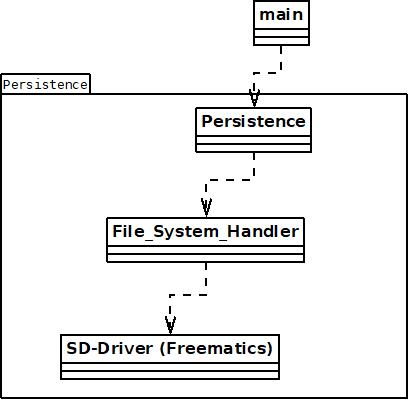
\includegraphics[scale=0.75]{./img/Persistence.jpg}
    \caption{Hierarchie beim SD Zugriff}
    \label{fig:Persistence}
  \end{center}
\end{figure}
Die Aufteilung in die oben gezeigten Klassen hat aber nicht nur eine bessere Lesbarkeit zu Folge. Ein weiterer Vorteil ist auch, eine bessere Trennung der Funktionalitäten voneinander. Den zwei Klassen \texttt{Persistence} und \texttt{File\_System\_Handler} sind folgende Aufgaben zugeteilt:\pagebreak
\subsubsection*{File\_System\_Handler Klasse}
Wie in Abbildung \ref{fig:Persistence} zu sehen ist, greift diese Klasse direkt auf den SD-Kartentreiber zu. Der \texttt{File\_System\_Handler} bietet die Möglichkeit mit von außen aufrufbaren Funktionen Dateien zu erstellen, zu öffnen, zu löschen und anzulegen. Diese Klasse sollte im Gesamtsystem nur einmal vorkommen, da sie eine Menge an Speicherplatz benötigt und der RAM auf dem \textit{ATmega328p} auf 2KB beschränkt ist.\cite{Atmega328P} Die Implementierung eines Singelton Patterns erfolgte nicht um zusätzlich benötigten Speicherplatz zu vermeiden.
Des weiteren ist es pro File\_System\_Handler nur möglich eine einzige Datei zu öffnen und nicht mehrere auf einmal. Auch das ist eine Schutzmaßname um unnötige Speicherplatz Verschwendung zu verhindern.
\subsubsection*{Persistence Klasse}
Da die erstellten Log-Dateien immer nach einem bestimmten Schema aufgebaut sind, kapselt die Klasse \texttt{Persistence} den \texttt{File\_System\_Handler} in sich. Um Daten zu schreiben erfolgt der Zugriff also immer über die Persistence Klasse und nicht über den \texttt{File\_System\_Handler} selbst. Dieser Mechanismus stellt sicher, dass die erstellten Log-Dateien immer den selben Format entsprechen. Einheitlich formatierte Dateien stellen sicher, dass eine Verarbeitung der geloggten Daten von den anderen Elementen des Systems, wie Backend und App, immer möglich ist.
\subsubsection*{Logging Format}
Wie im obigen Abschnitt bereits erwähnt zeichnen sich gute Log-Dateien durch ein einheitliches Format aus. Doch nicht nur eine einheitliche Formatierung spielt beim SmartCar eine Rolle, sondern auch der Speicherbedarf. So muss bei der Erfassung der Daten in einem kompakter Format erfolgen. Dieses Anforderung folgt schon alleine aus der Tatsache, dass es möglich sein soll, die geloggten Daten von dem Dongle über Bluetooth Low Energy(BLE) zu übertragen. Wären die Daten übermäßig groß, müsste ein Nutzer lange Zeit für den Transfer der Daten warten, was die Nutzbarkeit dieses Features beeinträchtigen würde. Aus diesen Gründen wurde das Datenformat aus Abbildung \ref{fig:LoggingEntry} für das Logging gewählt:
\begin{figure}[H]
\begin{center}
  \begin{tabular}{ | c || c | c | c | c |}
    \hline
    \textbf{Byte} & 1. & 2. - 9. & 10. - 11. & 12. - 15. \\ \hline
    \textbf{Wert} & MVID & Datum(ms) & Daten ID & Datenwert \\
    \hline
  \end{tabular}
  \caption{Format eines Logging Eintrags auf der SD-Karte (15Byte)}
  \label{fig:LoggingEntry}
\end{center}
\end{figure}
\subsubsection*{MVID}
Das erste Byte des Eintrags beschreibt die gemappte Fahrzeugnummer. Dieser Eintrag ist wichtig um die bei Verwendung des Dongles in mehreren Fahrzeugen die einzelnen Fahrzeuge und die einzelnen Routen auseinander zu halten. MVID ist eine fortlaufende Nummer von 0 bis 255 die bei jedem Einschalten des Fahrzeugs um eine Stelle erhöht wird. Die definierten 8 Bit stellen einen ausreichenden Zahlenraum dar, um ein komfortables Fahrtenmanagement zu gewährleisten. 
\subsubsection*{Datum}
Die nächsten 8 Byte beinhalten den Zeitstempel des Erfassten Wertes. Dieser wird in Millisekunden seit 01. Januar 1970 angegeben. Die Zeit ist einer der wichtigsten Werte für das Loggen, da nur so bei späteren Analysen festgestellt werden kann wann der Wert aufgenommen wurde. Der Zahlenbereich wurde auf 64 Bit festgelegt, da ein 32-Bit Wert nur bis ungefähr 2038 zählen könnte. Mit 64 Bit lässt sich ein weitaus größerer Zeitraum abdecken.
\subsubsection*{Daten ID}
Der 3. Wert is die ID des geloggtem Datums und liegt im 10. und 11. Byte. Dieser Wert richtet sich nach der in Abschnitt \ref{sec:systemDesign} gezeigten OBD-Tabelle. Zusätzlich zu den OBD-IDs kann dieses Feld Werte für die GPS-Koordinaten, den Beschleunigungssensor und das Gyroskop annehmen.  Nur mit der zugehörigem ID kann dem Wert eine Bedeutung zugeteilt werden. 
\subsubsection*{Wert}
Die letzten 4 Bytes des Eintrags beinhalten den eigentlichen erfassten Wert. Je nach ID muss dieser Wert anders interpretiert werden.
\subsection{Bluetooth Kommunikation}
\label{sec:Bluetooth}
Wie dem Kapitel \ref{sec:useCases} besteht die Möglichkeit mit dem Dongle über Bluetooth mit einer Smartphone App zu kommunizieren. Hierfür wird der Freematics ONE mit dem Bluetooth Low energy fähigem CC2541 Modul von Texas Instruments ausgeliefert.
\begin{figure}[H]
  \begin{center}
    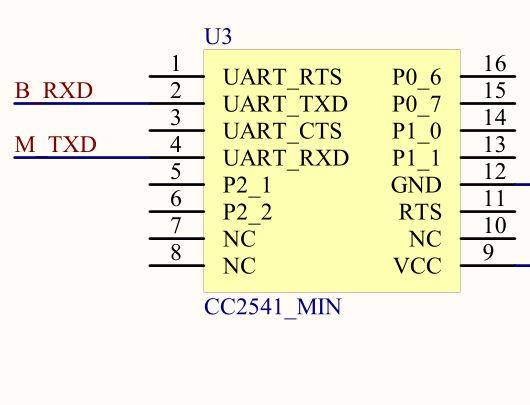
\includegraphics[scale=0.5]{./img/BLEChip.jpg}
    \caption{Schematischer Aufbau des CC2541\cite{Freematics2016}}
    \label{fig:BLEChip}
  \end{center}
\end{figure} 
Abbildung \ref{fig:BLEChip} zeigt den schematischen Aufbau des Chips und seine PINs. Die zwei UART Pins des Chips(UART\_TXD/UART\_RXD) sind mit den UART Pins des ATmega328p(B\_RXD/M\_TXD) verbunden. Der CC2541 ist so konfiguriert, dass jede Nachricht die von dem Mikrocontroller über UART versendet wird direkt über Bluetooth nach Außen gesendet wird. Dadurch entsteht der Effekt, dass für Nachrichten, die über die der Dongle über die Arudino Funktion \texttt{Serial.println()} ausgibt, automatisch ein Versenden über BLE erfolgt.
\paragraph{}{}
Aus diesem Grund gibt es beim SmartCar Code keine eigene Driver Schicht für die Bluetooth Kommunikation, denn diese ist bereits in den Arduino Bibliotheken implementiert. Der Dongle nutzt Bluetooth um die folgenden 2 Funktionen auszuführen.
\subsubsection*{1. Live Daten Übertragung}
Um Verschiedene Daten der OBD Schnittstelle während der Fahrt zu visualisieren besteht eine Verbindung der APP mit dem Dongle über Bluetooth. Der Dongle sendet bestimmte Daten nach dem Auslesen über Bluetooth zur App.
\begin{figure}[H]
\begin{center}
  \begin{tabular}{ | c | c | c | c | c |}
    \hline
    Startzeichen & ID & Trennzeichen & Wert & Endzeichen \\ \hline
    \# & uint16 & : & uint32 & ; \\
    \hline
  \end{tabular}
  \caption{Format einer Livedaten Nachricht}
  \label{fig:LiveDataMessage}
\end{center}
\end{figure}
Eine Live Daten Nachricht, wie in Abbildung \ref{fig:LiveDataMessage} zu sehen gliedert sich in folgende Teile:
\begin{enumerate}
  \item Start der Nachricht\textbf{(\#)}: Eine Raute am Anfang der Nachricht signalisiert, dass es sich bei dieser Nachricht um eine Live-Daten Nachricht handelt. Dieses Markieren verhindert ein versehentliches interpretieren eine anderen Nachricht als Live-Daten Nachricht.
  \item Daten ID: Direkt nach der Raute folgt die ID des Wertes der in der in der Nachricht enthalten ist. Sie richtet sich wieder nach den OBD-IDs aus Abschnitt \ref{sec:systemDesign}
  \item Trennzeichen(\textbf{:}): Nach der ID kommt ein Doppelpunkt als Trennzeichen
  \item Wert mit \textbf{;} am Ende: Als letztes enthält die Nachricht der Wert zur ID gefolgt von einem Strichpunkt und einem Zeilenumbruch 
\end{enumerate}
\pagebreak
\subsubsection*{2. Upload der Logdateien}
Die zweite Funktion des Dongles, die Bluetooth benötigt ist der Upload der geloggten Daten zum Smartphone. Der Dongle sendet hier nach einem Signal des Smartphones auf Nutzerwunsch Daten von der SD-Karte zur App. Dieses verfahren ist ein zweiter Weg um die Daten vom Dongle ins Backend zur Analyse zu befördern. Das Diagramm in Abbildung \ref{fig:DataUpload} zeigt den Ablauf einer solchen Datenübertragung zwischen App und Dongle. 
\begin{figure}[h]
  \begin{center}
    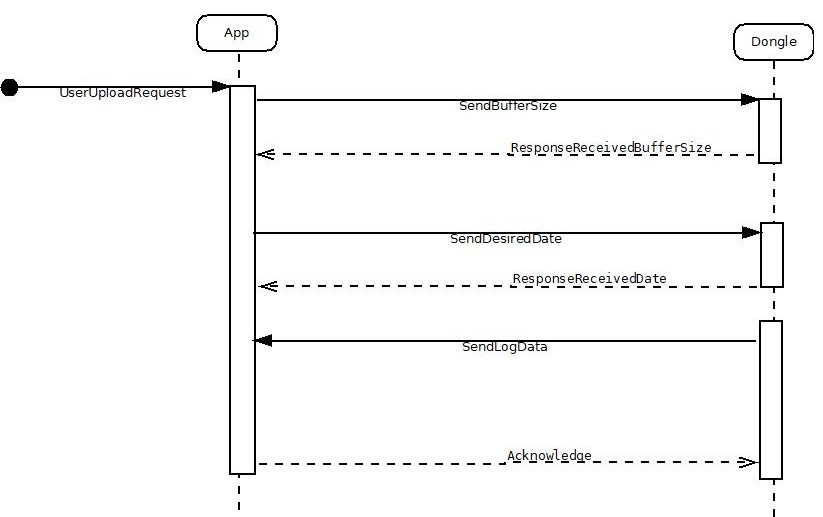
\includegraphics[scale=0.6]{./img/DataUploadSequence.jpg}
    \caption{Ablauf des Datenuploads via Bluetooth}
    \label{fig:DataUpload}
  \end{center}
\end{figure}

Der Ablauf lässt sich in 4 Teile unterteilen:
\begin{enumerate}
  \item Nutzer Request: Der Vorgang des Datenübertragens erfolgt mit der Interaktion des Nutzers auf dem Smartphone. 
  \item Übertragen der Puffer Größe: Nach der Anfrage des Nutzers sendet die App eine Puffer Größe an den Dongle. Diese Zahl stellt die Maximale Anzahl an Logeinträgen dar, die gesendet werden sollen. Diese Nachricht beginnt mit zwei Raute Zeichen(ASCII) gefolgt von einem 8-Bit Wert für den Puffer. Der Dongle bestätigt den Empfang des Puffers mit dem Zurücksenden der gleichen Nachricht. So kann die App sicherstellen, dass für die Pufferübertragung kein Fehler passiert ist. Für eine Puffergröße von 55 würde die Nachricht als String folgendermaßen aussehen: \#\#7 (7 $\equiv$ ASCII 55)
  \item  Mitteilen des Datums: Nach dem Empfang der Antwort des Dongles sendet die App dann das Datum zu dem die Daten übertragen werden sollen. Hier beginnt die Nachricht mit zwei Stichpunkten(ASCII) gefolgt von dem Datum(ASCII) im Format DDMMYYYY. Nach Empfang der Nachricht antwortet der Dongle wie bei der Puffergröße mit der gleichen Nachricht. Für den 01. Januar 2017 wäre die Nachricht ;;01012017
  \item Datenübertragung: Nach dem Austausch der nötigen Informationen beginnt der Dongle mit dem Senden der Daten bis die in 1. definierte Pufffergröße erreicht wurde, oder keine Logdaten mehr vorhanden sind.
\end{enumerate}


  

 
 
 
 
 
 
 
 
\chapter{Tests}
\label{sec:test}

\section{Dongle}
\label{sec:dongleTest}
Nach der erfolgreichen Integration der Dongle-Software erfolgte die Testphase, bei der der Dongle in iterativen Durchgängen an die OBD-Buchse verschiedener PKWs angeschlossen wurde. Hierbei wurden mehrere Fehlfunktionen entdeckt und behoben.
\paragraph{}
Es wurde zunächst deutlich, dass die Dauer der einzelnen Durchgänge der Haupt-Schleife weit über das erwartete Maß hinaus geht. Hierbei wurden die Zeitstempel zweier geloggter OBD-Werte mit der PID 0x0C verglichen. Dieser Wert ist der erste, der in jedem Durchgang erfasst wird. Folgende Werte zeigen beispielhaft die Dauern von Durchgänge bei denen alle Logging-Kategorien mindestens einmal erfasst wurden:
\begin{table}
  \caption{Beispiel-Zeiten für einzelne Durchgänge der Haupt-Schleife}
  \label{tab:loopTimes}

  \begin{center}
    \begin{tabular}{|c|c|c|}
    \hline
      Durchgang & Dauer in Millisekunden & erfasste Logging-Kategorien\\ \hline
      0 & 488 & A\\ \hline
      1 & 708 & A + B\\ \hline
      2 & 960 & A + C\\ \hline
      3 & 608 & A + D\\ \hline
      4 & 656 & A + B\\ \hline
    \end{tabular}
  \end{center}
\end{table}
Eine Analyse zeigte auf, dass diese hohen Zeiten vor allem durch die Latenz bei der Abfrage der OBD-Daten vom Steuergerät zustande kommen. Dieses Verhalten kann nicht beeinflusst werden, stellt allerdings nur ein kleines Problem dar. Da zu jedem erfassten Wert auch ein Zeitstempel mit einer Genauigkeit von \textpm 8 Millisekunden gespeichert wird, ist die Einhaltung der angestrebten 500 Millisekunden für spätere Berechnungen nicht notwendig. Die Unterschiedliche Frequenz mit der die Logging-Klassen erfasst werden, welche mittels der Modulo-Operationen auf dem Loop-Counter erreicht wird, bleibt aufgrund der geringen Änderungsrate der Werte jedoch bestehen.
\paragraph{}
Darüber hinaus zeigten die Tests, dass die Verwendung des LowPowerModes des Coprozessors nicht den Erwartungen entsprach. Der STM32 konnte zwar in einen Schlafzustand versetzt werden, die Reaktivierung des selben konnte jedoch trotz intensiver Recherche im veröffentlichten Code und im offiziellen Freematics Forum nicht erreicht werden. Es zeigte sich allerdings, dass die verwendeten Funktionen aus den aktuelleren Versionen der offiziellen Softwarebibliotheken entfernt wurden \cite{freematicsRevFeb}. Da bereits ein Timeout bei der Abfrage von OBD-Werten dazu führt, dass die Dongle-Software ein Abstellen des Fahrzeuges vermutet, folgte daraus ein zufälliges Abbrechen der Aufzeichnung während einer laufenden Fahrt. Zur Beseitigung des Problems wurde auf die Verwendung des LowPowerModes verzichtet. Dieses Problem stellt im aktuellen Projektstand eine Verbesserungsmöglichkeit dar.

\chapter{Ausblick}
\label{sec:outlook}
Aufgrund der beschränkten Ressourcen die für dieses Projekt zur Verfügung standen, konnte das Potential des zuvor vorgestellten Systems bei weitem noch nicht ausgeschöpft werden. Aus diesem Grund, soll das folgende Kapitel Ideen vermitteln was beispielsweise mit der Infrastruktur darüber hinaus erreicht werden kann.

\section{Identifikation des Fahrers}
Mithilfe der aufgezeichneten Beschleunigungsdaten wäre es möglich die Infrastruktur dementsprechend zu erweitern, dass aus den aufgezeichneten Daten personalisierte Fahrtenbücher auch ohne die Notwendigkeit für ID Karten oder sonstige Mittel zur Identifikation des Fahrers erstellt werden können. Dies würde vermutlich funktionieren, da jeder Fahrer seinen eigenen persönlichen Fahrstil besitzt der z.B. das Anfahren und Abbremsen beeinflusst.
\\
Diese Möglichkeit der Identifikation hätte den Vorteil, dass auch nachträglich festgestellt werden kann wer der Fahrer war.

\section{Bewertung des Fahrverhaltens}
Ebenso wäre es mit den aufgezeichneten Daten möglich den Fahrstil der Fahrer zu bewerten. Wird beispielsweise an der Ampel mit dem Gas gespielt oder der Drehzahlbereich jedes mal bis zum roten Bereich ausgelastet?
\\
Diese Daten wären zum einen z.B. für Versicherungen oder Firmen interessant, können allerdings auch Privatpersonen helfen z.B. herauszufinden wer der anderen Mitfahrer für den schnelleren Verschleiß von Reifen oder anderer Teile zuständig sein könnte.

\section{Ermittlung von Engpässen}
\label{SecErmittlungVonEngpaessen}
Alleine mit den aufgezeichneten GPS-Daten ist es möglich Engpässe im Straßennetz zu erkennen und dagegen entsprechende Gegenmaßnahmen in die Wege zu leiten (z.B. Ausbau von Straßen, Ampelanlagen zeitlich anders schalten, ...).
\\
Weiterhin wäre eine solche Analyse z.B. auch für Firmen hilfreich. Dies würde nicht dazu führen, dass das Straßennetz geändert würde, aber die Fahrer könnten alternative Routen vorgeschlagen bekommen welche weniger frequentierte Strecken nutzen.
\\
Jede dieser Möglichkeiten würde auf Dauer dazu führen, dass sich die Verkehrslage entspannen kann.

\section{Erstellung von Spritsparrouten}
Die in Kapitel \ref{SecErmittlungVonEngpaessen} vorgestellten Ideen könnten weiterhin verwendet werden um Routen zu finden bei denen der Fahrer aufgrund von weniger Stop and Go Verkehr Sprit einsparen kann.

\section{Softwareoptimierungen}
Wie bereits in Kapitel \ref{sec:dongleTest} aufgezeigt wurde, besteht immer noch Potential, um den Dongle auf Energiesparmöglichkeiten zu untersuchen und diese zu implementieren. Zudem ist die weitere Optimierung des Codes auf RAM-Größe noch empfehlenswert, um die Probleme aus Kapitel \ref{subsec:intPl} zu beheben.

\section{Bluetooth Flashtool}
\label{sec:appAusblick}
Um den Atmega328P Chip neu zu programmieren muss bis jetzt auf die USB-UART Schnittstelle zurückgegriffen werden. Dieses Vorgehen ist relativ umständlich, da das Flashen über einen Desktop-PC mit der gesamten Toolchain geschehen muss. Um diesen Prozess zu erleichtern besteht die Möglichkeit die App mit einer Bluetooth Flasher Funktion zu erweitern.
\paragraph{}
Wie bereits in Kapitel \ref{sec:Bluetooth} dargestellt, ist der Bluetooth Chip direkt mit dem Seriellen UART-Interface des Atmega328P Chips verbunden. Da der CC2541 unabhängig vom Atmega328P läuft, kann diese Tatsache ausgenutzt werden um den Atmel Chip direkt über Bluetooth zu flashen. Ein solches Feature in der App erleichtert das Ausrollen von neuen Sofware Updates sehr.
\paragraph{}
Der Nutzer müsste hier nur den neuen Programmcode auf sein Smartphone laden und könnte dann den Dongle neu flashen.
Daraus entstünden die folgenden Vorteile:
\begin{enumerate}
	\item App-Software und Dongle-Software können immer gleichzeitig aktualisiert werden und passen so jeder Zeit zueinander
	\item Jeder Nutzer kann den Dongle mit einem Smartphone neu flashen. Ein Bugfix kann so schnell ausgerollt werden
\end{enumerate}


\newpage
\listoffigures
\lstlistoflistings
\listoftables
% Muss von Hand sortiert werden!!

%anlegen:
% \acro{}[]{}
% \acro{}{}

%verwenden
%\ac{x} dann wird x als verlinkung genommen  
%\acp{x} wird auch x als verlinkung genommen, aber mit einem s am ende für mehrzahl

%\newpage
\section*{Abkürzungsverzeichnis} %Abkürzungsverzeichnis
\markboth{Abkürzungsverzeichnis}{}
\begin{acronym}[ABCDEFGHIJK] 			% längste Abkürzung steht in eckigen Klammern
	\acro{GPS}{Global Positioning System}
	\acro{MEMS}{Microelectromechanical System}
	\acro{NMEA}{National Marine Electronics Association}
  	\acro{API}{Application Programming Interface}
	\acro{OBD}{On Board Diagnistic}
	\acro{PID}{Parameter Identifikator}
	\acro{SBAS}{Satellite-based augmentation systems}
	\acro{UART}{Universal asynchronous receiver-transmitter}
	\acro{VIN}{Vehicle Identification Number}
	\acro{BLE}{Bluetooth Low Energy}
	\acro{MVID}{Mapped Vehilce Identification Number}
	\acro{RAM}{Random Access Memory}
	\acro{LINQ}{Language Integrated Query}
\end{acronym}

\printbibliography

\newpage
\appendix










\end{document}